\section{Code Verification} % (fold)
\label{sec:code_verification}

	\subsection{Rayleigh B\`enard Convection} % (fold)
	\label{sub:rayleigh_b_enard_convection}
	
		We verify our code by comparing to the well tested case of Rayleigh B\`enard convection.
			We solve the traditional nondimensional Rayleigh B\`enard convection equations:
			\begin{align}
				\frac{1}{\rm{Pr}}\left(\frac{\partial{\vect{u}}}{\partial{t}}+\vect{u}\cdot\nabla{\vect{u}}\right)&=-\nabla{p}+\rm{Ra}T+\nabla^{2}\vect{u},\\
				\frac{\partia{T}}{\partial{t}}+\vect{u}\cdot\nabla{T}&=\nabla^{2}T.
			\end{align}
			Unlike most solutions in the literature, we solve this with our predictor-corrector algorithm rather than by constructing a stream function to enforce incompressibility (see Section \ref{incompressible}).
		
		We compare to the results from \citet{Moore1973} by running a two-dimensional test case with aspect ratio of 2.828 and $\rm{Pr}$ of 6.8.
			We present the results in Figure \ref{rbconvection}, where it can be seen that ISCES can reproduce the results from the literature quite well.
			
		\begin{figure}[h]
		  \centering
		    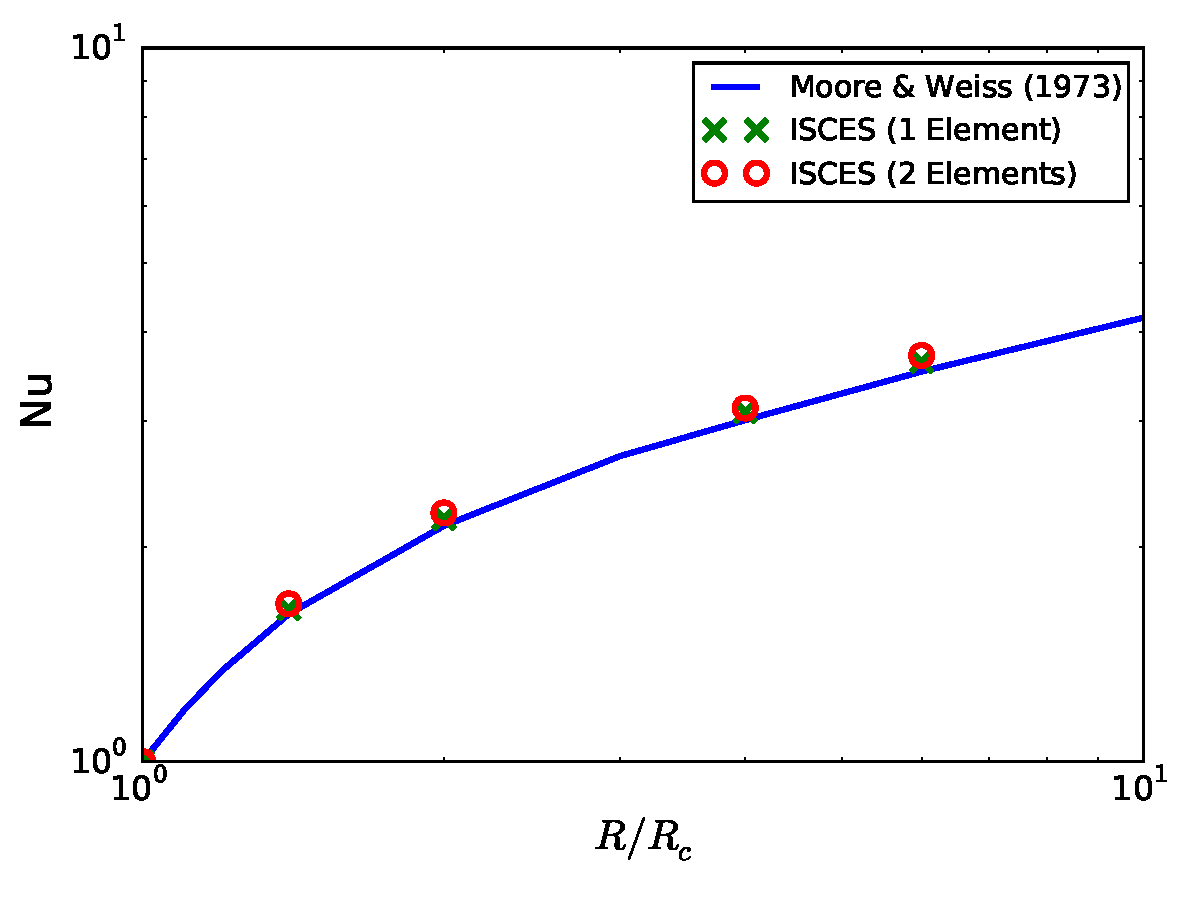
\includegraphics[width=.9\textwidth]{../figs/verify.pdf}
		  \caption{The Nusselt number (total flux divided by background diffusive flux) for simulations of varying Rayleigh number of ISCES compared to those from the literature. The abscissa has been scaled by the critical Rayleigh number for the system; for Prandtl number 6.8, this is approximately 657. The crosses represent ISCES run with a single element, and the circles, two elements. The solid line represent the results from \citet{Moore1973}.}
		  \label{fig:figs_verify}
		\end{figure}
	
	% subsection rayleigh_b_enard_convection (end)

% section code_verification (end)